
%%%%%%%%%%%%%%%%%%%%%%% file typeinst.tex %%%%%%%%%%%%%%%%%%%%%%%%%
%
% This is the LaTeX source for the instructions to authors using
% the LaTeX document class 'llncs.cls' for contributions to
% the Lecture Notes in Computer Sciences series.
% http://www.springer.com/lncs       Springer Heidelberg 2006/05/04
%
% It may be used as a template for your own input - copy it
% to a new file with a new name and use it as the basis
% for your article.
%
% NB: the document class 'llncs' has its own and detailed documentation, see
% ftp://ftp.springer.de/data/pubftp/pub/tex/latex/llncs/latex2e/llncsdoc.pdf
%
%%%%%%%%%%%%%%%%%%%%%%%%%%%%%%%%%%%%%%%%%%%%%%%%%%%%%%%%%%%%%%%%%%%


\documentclass[runningheads,a4paper]{llncs}

\usepackage{amssymb}
\setcounter{tocdepth}{3}
\usepackage{graphicx}

\usepackage{url}  
\newcommand{\keywords}[1]{\par\addvspace\baselineskip
\noindent\keywordname\enspace\ignorespaces#1}

\usepackage{nameref}
\begin{document}

\mainmatter  % start of an individual contribution

% first the title is needed
\title{DAT530\\Discrete Simulation and Performance Analysis\\Final Project\\Solitaire game strategy}

% a short form should be given in case it is too long for the running head
\titlerunning{DAT530 - Final Project}


\author{Racin W. Nygaard}%

%
\authorrunning{DAT530 - Final Project - Solitaire game strategy}
% (feature abused for this document to repeat the title also on left hand pages)

% the affiliations are given next; don't give your e-mail address
% unless you accept that it will be published
\institute{Universitetet i Stavanger}

%
% NB: a more complex sample for affiliations and the mapping to the
% corresponding authors can be found in the file "llncs.dem"
% (search for the string "\mainmatter" where a contribution starts).
% "llncs.dem" accompanies the document class "llncs.cls".
%

\toctitle{Solitaire game strategy}
\tocauthor{Report}
\maketitle


\begin{abstract}
SKRIV DETTE TIL SLUTT!

\end{abstract}


\section{Introduction}
This project aims to study the popular card game, Solitaire[Site]. Solitaire is bundled with most Windows[Site] installations, as well as being available for free on several sources. It is also easy to play the game with a physical card deck. A detailed explaination of the games rules can be found in the next chapter, Solitaire Rules[REF]
\newline
Since the game utilizes all 52 cards of the deck, the number of possible initial game states is 52!, which is a very high number. A large number of these inital game states can be merged, as they offer no difference in the difficulty to solve. Some of these intial states are unsolvable, but even given a solvable game state, one often find oneself in an unsolvable game state, due to certain actions in the game are non-reversible,. There has been attempts to find the distribution of solvable and unsolvable initial game states [ref]. This is roughly 75 percent are solvable, however the study also shows that only 35 percent of the games are won by an experienced player.
\newline
This project contains a complete model of the game, a GUI to play the game, and a basic bot to simulate user actions. 

\subsection{Solitaire Rules}

Finite State Machine ?


\section{Method and Design}
\label{sec:2_method_and_design}
\subsection{Overall Design}
The model developed is pretty large, and contains 99 transition and 88 places. It is developed using the modualar approach, and encompasses 6 different modules. Some of the modules are duplicated, with the only difference being the names of the transitions and places.
\begin{center}
	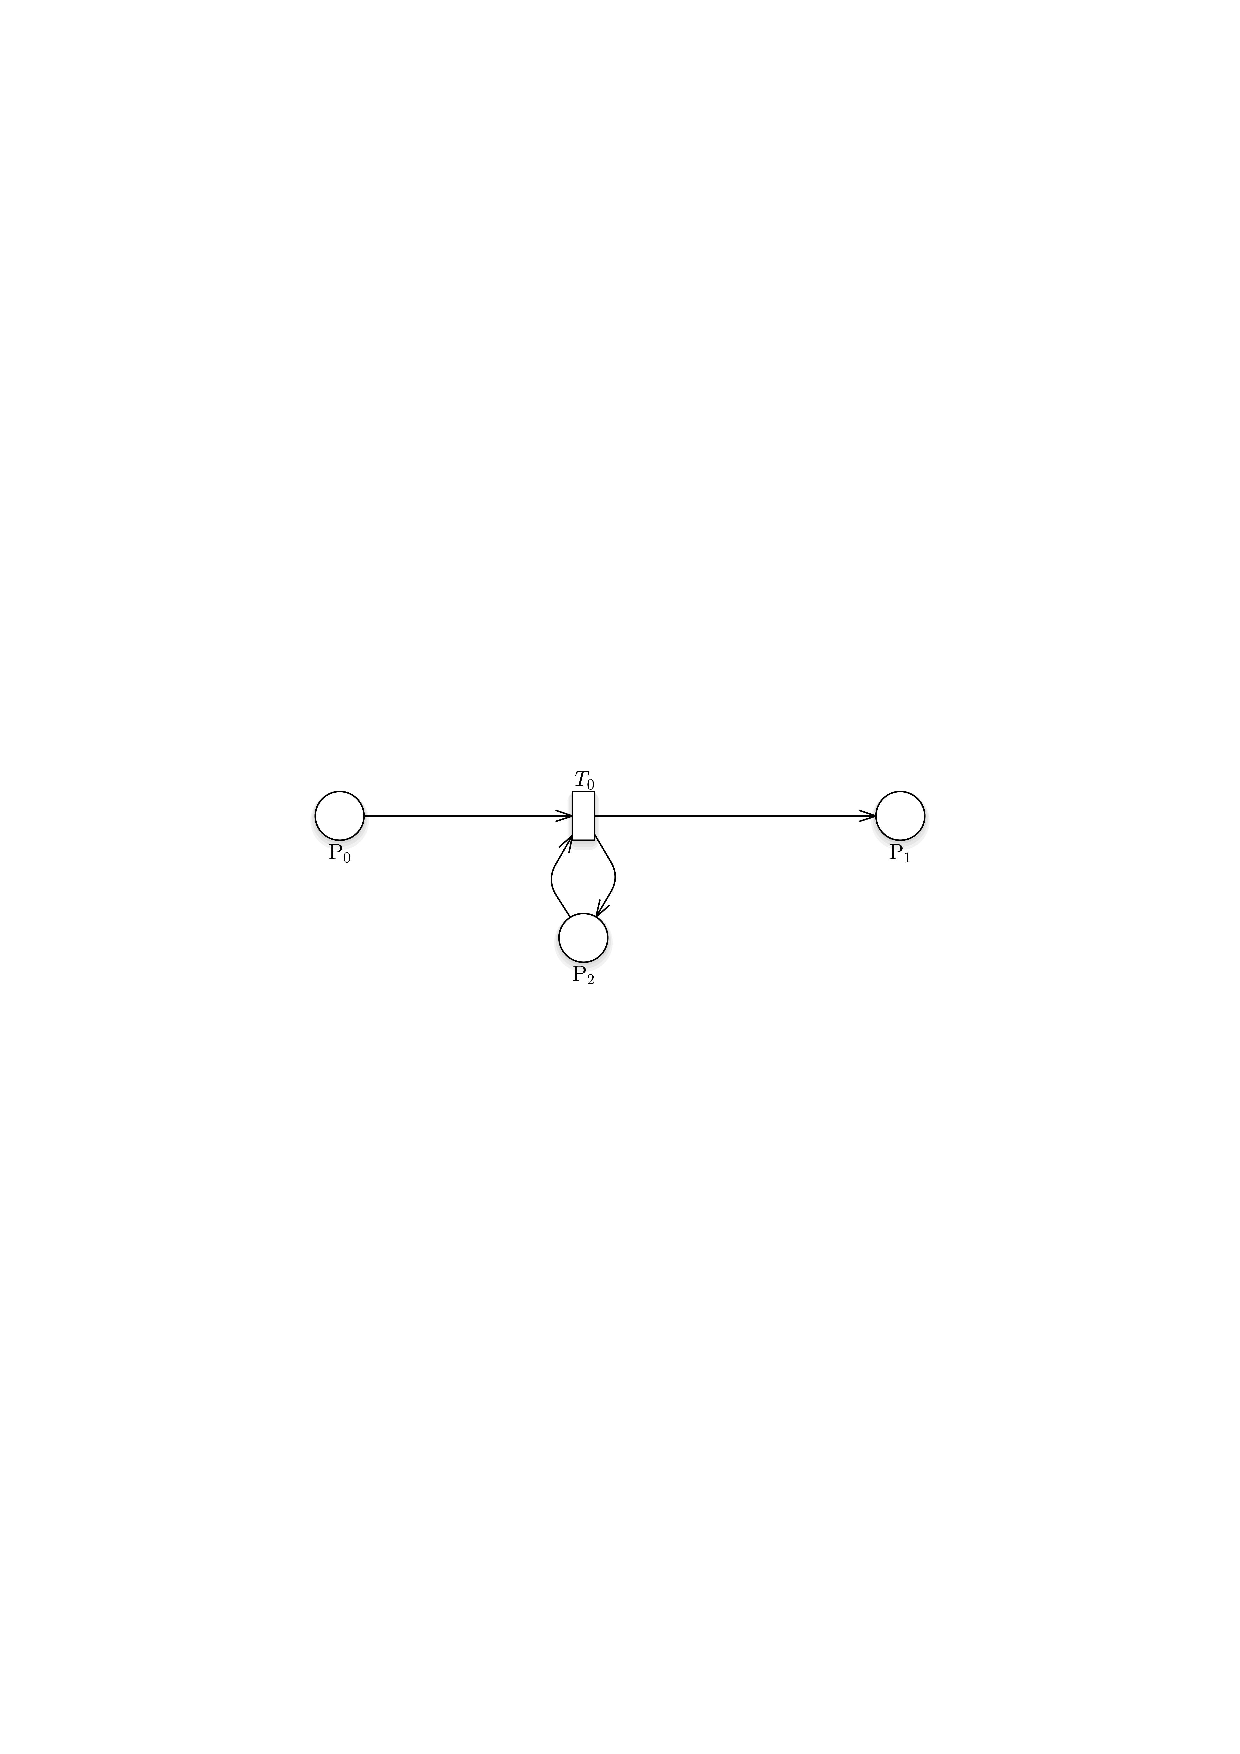
\includegraphics[width=\textwidth]{images/test}
\end{center}
\subsection{Draw Pile Module}
The Draw Pile module has several key responsibilities. When first running the model, it will use the initial tokens of [Place] and give each of them a color according to [LIST]. If the [RANDOM_OPTION] is set, the cards are randomly dealt.
\subsection{Foundation Pile Module}
\subsection{Tableau Pile Module}
\subsection{Module Connector Module}
\subsection{Player Module}
\subsection{Player Bot Module}





\section{Implementation}
\label{sec:3_implementation}
\subsection{Algorithms}
\subsubsection{Atomicity}
In order to preventdd
\subsection{Initial Dealing}
\subsection{Resources}
\subsection{Moving Multiple Cards}

\begin{verbatim}
    def mapper_from_to(self, key, email):
        if 'to' in email.keys() and 'from' in email.keys() and 'body_count' in email.keys():
\end{verbatim}

\section{Testing, Analysis and Results}
\label{sec:3_implementation}
\subsection{Algorithms}
\subsubsection{Atomicity}
In order to preventdd
\subsection{Initial Dealing}
\subsection{Resources}
\subsection{Moving Multiple Cards}

\section{Discussion}



% Keeping this for reference for now %
\begin{thebibliography}{7}

\bibitem{wikiTFIDF} Wikipedia article on Tf-idf. \url{https://en.wikipedia.org/wiki/Tf?idf}
\bibitem{oreilly} Tom White, Hadoop: The Definitive Guide, 2015, \emph{ISBN: 978-1-491-90163-2}
\bibitem{dockerdocs} Docker API Docs, \url{https://docs.docker.com}
\bibitem{dat630slides} Slides from DAT630, Krisztian Balog
\bibitem{dataset} Kaggle. The Enron Email Dataset. \url{https://www.kaggle.com/wcukierski/enron-email-dataset}
\bibitem{coursematerial} Data Intensive Systems Compendium, Tomasz Wiktorski et al.
\bibitem{git} Source code of all tasks developed. GitLab \url{https://gitlab.com/mindejulian/projectDAT500/tree/master}

\end{thebibliography}

\end{document}
